% This file was created by tikzplotlib v0.9.4.
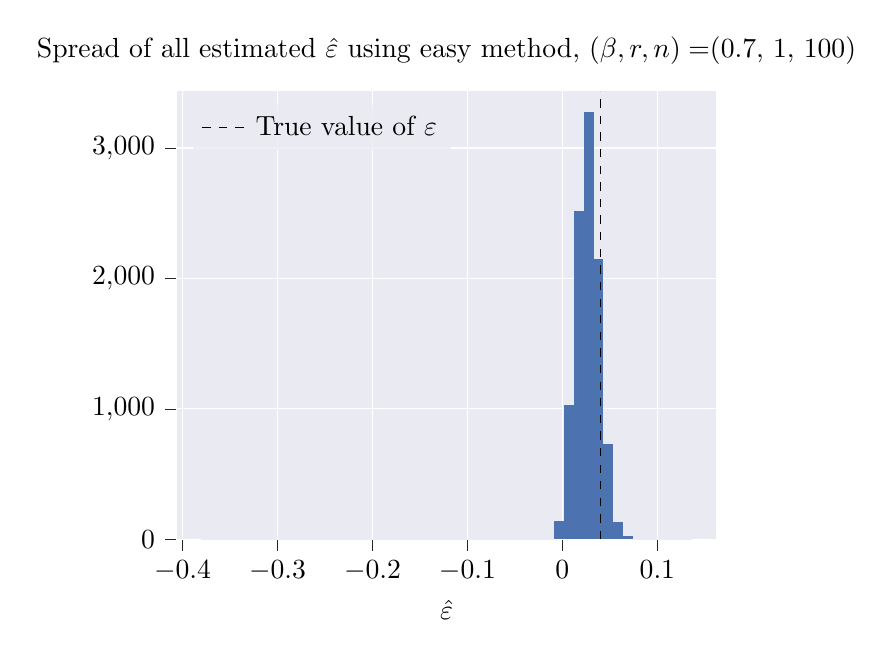
\begin{tikzpicture}

\definecolor{color0}{rgb}{0.917647058823529,0.917647058823529,0.949019607843137}
\definecolor{color1}{rgb}{0.298039215686275,0.447058823529412,0.690196078431373}

\begin{axis}[
axis background/.style={fill=color0},
axis line style={white},
legend cell align={left},
legend style={fill opacity=0.8, draw opacity=1, text opacity=1, at={(0.03,0.97)}, anchor=north west, draw=none, fill=color0},
tick align=outside,
tick pos=left,
title={Spread of all estimated \(\displaystyle \hat{\varepsilon}\) using easy method, \(\displaystyle (\beta,r,n) = \)(0.7, 1, 100) },
x grid style={white},
xlabel={\(\displaystyle \hat{\varepsilon}\)},
xmajorgrids,
xmin=-0.406235675348165, xmax=0.162080149677429,
xtick style={color=white!15!black},
y grid style={white},
ymajorgrids,
ymin=0, ymax=3437.7,
ytick style={color=white!15!black}
]
\draw[draw=none,fill=color1,line width=0.12pt] (axis cs:-0.380403137847001,0) rectangle (axis cs:-0.370070122846536,0);
\draw[draw=none,fill=color1,line width=0.12pt] (axis cs:-0.370070122846536,0) rectangle (axis cs:-0.359737107846071,0);
\draw[draw=none,fill=color1,line width=0.12pt] (axis cs:-0.359737107846071,0) rectangle (axis cs:-0.349404092845605,0);
\draw[draw=none,fill=color1,line width=0.12pt] (axis cs:-0.349404092845605,0) rectangle (axis cs:-0.33907107784514,0);
\draw[draw=none,fill=color1,line width=0.12pt] (axis cs:-0.33907107784514,0) rectangle (axis cs:-0.328738062844675,0);
\draw[draw=none,fill=color1,line width=0.12pt] (axis cs:-0.328738062844675,0) rectangle (axis cs:-0.318405047844209,0);
\draw[draw=none,fill=color1,line width=0.12pt] (axis cs:-0.318405047844209,0) rectangle (axis cs:-0.308072032843744,0);
\draw[draw=none,fill=color1,line width=0.12pt] (axis cs:-0.308072032843744,0) rectangle (axis cs:-0.297739017843278,0);
\draw[draw=none,fill=color1,line width=0.12pt] (axis cs:-0.297739017843278,0) rectangle (axis cs:-0.287406002842813,0);
\draw[draw=none,fill=color1,line width=0.12pt] (axis cs:-0.287406002842813,0) rectangle (axis cs:-0.277072987842348,0);
\draw[draw=none,fill=color1,line width=0.12pt] (axis cs:-0.277072987842348,0) rectangle (axis cs:-0.266739972841882,0);
\draw[draw=none,fill=color1,line width=0.12pt] (axis cs:-0.266739972841882,0) rectangle (axis cs:-0.256406957841417,0);
\draw[draw=none,fill=color1,line width=0.12pt] (axis cs:-0.256406957841417,0) rectangle (axis cs:-0.246073942840952,0);
\draw[draw=none,fill=color1,line width=0.12pt] (axis cs:-0.246073942840952,0) rectangle (axis cs:-0.235740927840486,0);
\draw[draw=none,fill=color1,line width=0.12pt] (axis cs:-0.235740927840486,0) rectangle (axis cs:-0.225407912840021,0);
\draw[draw=none,fill=color1,line width=0.12pt] (axis cs:-0.225407912840021,0) rectangle (axis cs:-0.215074897839556,0);
\draw[draw=none,fill=color1,line width=0.12pt] (axis cs:-0.215074897839556,0) rectangle (axis cs:-0.20474188283909,0);
\draw[draw=none,fill=color1,line width=0.12pt] (axis cs:-0.20474188283909,0) rectangle (axis cs:-0.194408867838625,0);
\draw[draw=none,fill=color1,line width=0.12pt] (axis cs:-0.194408867838625,0) rectangle (axis cs:-0.18407585283816,0);
\draw[draw=none,fill=color1,line width=0.12pt] (axis cs:-0.18407585283816,0) rectangle (axis cs:-0.173742837837694,0);
\draw[draw=none,fill=color1,line width=0.12pt] (axis cs:-0.173742837837694,0) rectangle (axis cs:-0.163409822837229,0);
\draw[draw=none,fill=color1,line width=0.12pt] (axis cs:-0.163409822837229,0) rectangle (axis cs:-0.153076807836764,0);
\draw[draw=none,fill=color1,line width=0.12pt] (axis cs:-0.153076807836764,0) rectangle (axis cs:-0.142743792836298,0);
\draw[draw=none,fill=color1,line width=0.12pt] (axis cs:-0.142743792836298,0) rectangle (axis cs:-0.132410777835833,0);
\draw[draw=none,fill=color1,line width=0.12pt] (axis cs:-0.132410777835833,0) rectangle (axis cs:-0.122077762835368,0);
\draw[draw=none,fill=color1,line width=0.12pt] (axis cs:-0.122077762835368,0) rectangle (axis cs:-0.111744747834902,0);
\draw[draw=none,fill=color1,line width=0.12pt] (axis cs:-0.111744747834902,0) rectangle (axis cs:-0.101411732834437,0);
\draw[draw=none,fill=color1,line width=0.12pt] (axis cs:-0.101411732834437,0) rectangle (axis cs:-0.0910787178339716,0);
\draw[draw=none,fill=color1,line width=0.12pt] (axis cs:-0.0910787178339716,0) rectangle (axis cs:-0.0807457028335063,0);
\draw[draw=none,fill=color1,line width=0.12pt] (axis cs:-0.0807457028335063,0) rectangle (axis cs:-0.0704126878330409,0);
\draw[draw=none,fill=color1,line width=0.12pt] (axis cs:-0.0704126878330409,0) rectangle (axis cs:-0.0600796728325756,0);
\draw[draw=none,fill=color1,line width=0.12pt] (axis cs:-0.0600796728325756,0) rectangle (axis cs:-0.0497466578321102,0);
\draw[draw=none,fill=color1,line width=0.12pt] (axis cs:-0.0497466578321102,0) rectangle (axis cs:-0.0394136428316449,0);
\draw[draw=none,fill=color1,line width=0.12pt] (axis cs:-0.0394136428316449,0) rectangle (axis cs:-0.0290806278311795,0);
\draw[draw=none,fill=color1,line width=0.12pt] (axis cs:-0.0290806278311795,0) rectangle (axis cs:-0.0187476128307142,0);
\draw[draw=none,fill=color1,line width=0.12pt] (axis cs:-0.0187476128307142,0) rectangle (axis cs:-0.00841459783024884,0);
\draw[draw=none,fill=color1,line width=0.12pt] (axis cs:-0.00841459783024884,0) rectangle (axis cs:0.00191841717021646,143);
\draw[draw=none,fill=color1,line width=0.12pt] (axis cs:0.00191841717021646,0) rectangle (axis cs:0.0122514321706818,1030);
\draw[draw=none,fill=color1,line width=0.12pt] (axis cs:0.0122514321706818,0) rectangle (axis cs:0.0225844471711472,2515);
\draw[draw=none,fill=color1,line width=0.12pt] (axis cs:0.0225844471711472,0) rectangle (axis cs:0.0329174621716125,3274);
\draw[draw=none,fill=color1,line width=0.12pt] (axis cs:0.0329174621716125,0) rectangle (axis cs:0.0432504771720779,2151);
\draw[draw=none,fill=color1,line width=0.12pt] (axis cs:0.0432504771720779,0) rectangle (axis cs:0.0535834921725432,728);
\draw[draw=none,fill=color1,line width=0.12pt] (axis cs:0.0535834921725432,0) rectangle (axis cs:0.0639165071730086,134);
\draw[draw=none,fill=color1,line width=0.12pt] (axis cs:0.0639165071730086,0) rectangle (axis cs:0.0742495221734739,25);
\draw[draw=none,fill=color1,line width=0.12pt] (axis cs:0.0742495221734739,0) rectangle (axis cs:0.0845825371739392,0);
\draw[draw=none,fill=color1,line width=0.12pt] (axis cs:0.0845825371739392,0) rectangle (axis cs:0.0949155521744046,0);
\draw[draw=none,fill=color1,line width=0.12pt] (axis cs:0.0949155521744046,0) rectangle (axis cs:0.10524856717487,0);
\draw[draw=none,fill=color1,line width=0.12pt] (axis cs:0.10524856717487,0) rectangle (axis cs:0.115581582175335,0);
\draw[draw=none,fill=color1,line width=0.12pt] (axis cs:0.115581582175335,0) rectangle (axis cs:0.125914597175801,0);
\draw[draw=none,fill=color1,line width=0.12pt] (axis cs:0.125914597175801,0) rectangle (axis cs:0.136247612176266,0);
\addplot [black, dashed]
table {%
0.0398107170553498 1.13686837721616e-13
0.0398107170553498 3437.7
};
\addlegendentry{True value of $\varepsilon$}
\end{axis}

\end{tikzpicture}
